\documentclass[]{standalone}
\usepackage{mathptmx}
%\renewcommand{\familydefault}{\rmdefault}
\usepackage[T1]{fontenc}
\usepackage[latin9]{inputenc}
\usepackage{siunitx}
\usepackage{array}
\usepackage{amsmath}
\usepackage{ifthen}
\usepackage{pgfplots}
\pgfplotsset{compat=1.14}
\usepackage{titling, graphicx}
\usepackage{tikz}
\usepackage{upgreek}
\usepackage{amsmath,amsthm}
\usepackage{strtikz}
\usetikzlibrary{shapes,arrows.meta,intersections,graphs,graphs.standard,math,fit}
\usetikzlibrary{calc,intersections,through,backgrounds}
\usetikzlibrary{decorations.pathmorphing, decorations.markings,decorations.pathreplacing}


\begin{document}
\def \fsize {\tiny}
\begin{tikzpicture}
\bilinear[startx = 0cm,
	starty = 0cm,
	yield displacement = 1cm,
	yield force = 2cm,
	maximum displacement = 4cm,
	maximum force = 2.5cm,
	axis space = 1cm,
	mode = 8,
	x-axis label = {Disp., $(d)$},
	y-axis label = {Force, $(f)$},
	kp text = $k_\textrm{p}$,
	ks text = $k_\textrm{s}$,
	fy text = $f_\textrm{y}$,
	dy text = $d_\textrm{y}$,
	mark yield point = 1,
	fmax text = $f_\textrm{m}$,
	dmax text = $d_\textrm{m}$,
	mark max point = 1,
	axis line thickness = 1pt,
	line thickness = 1pt,
	show axes labels = 1,
	show stiffness = 1,
	show arrows = 0,
	show line arrows = 1,
	arrow length = 6pt,
	arrow width = 4pt]
%\draw (0,0) -- (1cm,1cm);
\end{tikzpicture}
\end{document}